%% ----------------------------------------------------------------
%% Experiment.tex
%% ---------------------------------------------------------------- 
\chapter{RetinaNet Deployment And Proposed Architectures} \label{Chapter:Experiment}
This chapter presents a detailed and analytical description of the system deployment, the proposed architectures and the hyper-parameter selection accompanied by the respective reasoning behind every choice. It is also investigated, how performance scales in function with the dataset training size. Finally, peak detection and counting is achieved by optimising the hyper-parameters of the final pipeline.

\section{Dataset Description}
The dataset used in the present thesis, was released in the work of \cite{bargoti2017image} and \cite{bargoti2017deep} and is provided through the Australian Centre or Field Robotics (ACFR), The University of Sydney\footnote{\url{http://data.acfr.usyd.edu.au/ag/treecrops/2016-multifruit/}}. The images were collected using the platform "Shrimp", an unmanned ground vehicle in apple, mango and almond orchards. However, in this study, only the apple subset is used.

Specifically, the dataset consists of random crops from images that span entire trees, trellised in the orchard block. The total number of apple instances in the images represents the total number of fruits in the orchard block. The split in training, validation and test set follows the proposed split from authors' previous work, to provide valid comparisons with the previous literature work. An overview of the dataset is presented in \tref{tab1}.

\begin{table}[!htb]
  \centering
  \resizebox{\textwidth}{!}{
  \begin{tabular}{cccccc}
  \toprule
  \textbf{Set} & \textbf{Raw Img. Size} & \textbf{Cropped Img. Size} & \textbf{No. of Img.} & \textbf{Fruit Width} & \textbf{Fruits/Img.} \\
  \midrule
  train 		& $1616\times1232$ & $202\times308$ & 896	& $36.27 \pm 7.55$  & $5.22 \pm 3.37$\\
  val. 		& $1616\times1232$ & $202\times308$ & 112 	& $35.92 \pm 7.83$  & $4.80 \pm 3.10$\\
  test. 		& $1616\times1232$ & $202\times308$ & 112 	& $35.29 \pm 7.30$  & $4.95 \pm 3.21$\\
  train + val. 	& $1616\times1232$ & $202\times308$ & 1008	& $36.23 \pm 7.58$	& $5.17 \pm 3.35$\\
  \bottomrule
  \end{tabular}
  }
  \caption{ACFR dataset description}
  \label{tab1}
\end{table}

The dataset provides circular annotations for the fruits; thus, they were converted to squares with the same width and height. Instead of discarding annotations that exceed the borders of the image, they were clipped to fit the image.
 
 \begin{figure}[!htb]
  \centering
  \subfigure[]{
    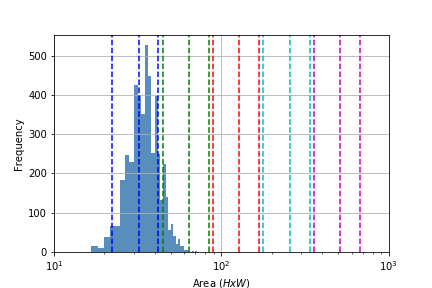
\includegraphics[width=0.30\textwidth]{figures/ch3/fig1_1.png}
    \label{fig1_1}
  }
  \subfigure[]{
    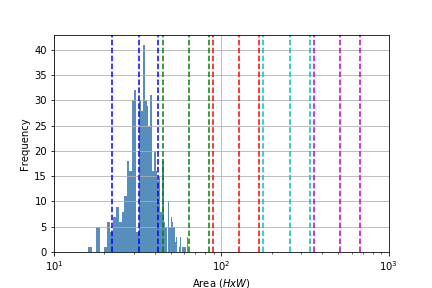
\includegraphics[width=0.30\textwidth]{figures/ch3/fig1_2.png}
    \label{fig1_2}
  }
  
    \subfigure[]{
    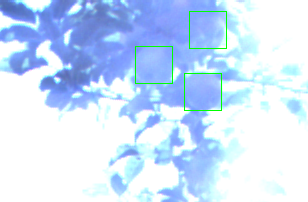
\includegraphics[width=0.30\textwidth]{figures/ch3/fig1_3.png}
    \label{fig1_3}
  }
  \subfigure[]{
    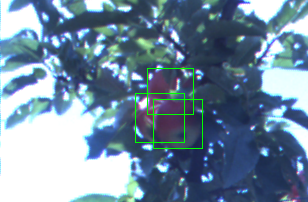
\includegraphics[width=0.30\textwidth]{figures/ch3/fig1_4.png}
    \label{fig1_4}
  }
  \caption{Typical samples from the ACFR dataset: A sample with (a) well-separated apples, (b) some unannotated instances and 
  		(c) poor lighting conditions. (d) NMS suppresses all predictions with $\text{IoU}\geq\text{NMS}_{th}$ apart from the one with the biggest confidence.}
  \label{fig1}
\end{figure}
 
\section{Proposed Deployment and Configuration}
\subsection{Hardware and Software specifications}
The deployment was set up on the Keras (\cite{chollet2015keras}) implementation of RetinaNet, provided by Fizyr\footnote{\url{https://github.com/fizyr/keras-retinanet}} and trained using a single NVIDIA GeForce GTX 1080 Ti provided by the Iridis 5\footnote{\url{https://www.southampton.ac.uk/isolutions/staff/iridis.page}} Computer Cluster. Appendix \ref{pack_versions} includes the complete list with the packages' versions. The repository can be found in \url{https://github.com/nikostsagk/Apple-detection}.

\subsection{Training Details}\label{training_details}
All models were trained on the complete training set, consisting of 896 images, while performance was monitored with respect to the validation set. Performance metrics presented below refer to the test set.

The models were trained for 30 epochs of 2000 steps each with $\text{batch size} = 1$. Regarding the optimiser, ADAM (\cite{kingma2014adam}) was used, with an initial learning rate of $10^{-5}$, decreased later by a factor of 10 on epoch 15 and again on 25. It was observed that the models did not exhibit any signs of overfitting as the performance on the validation set was increasing until it stabilised around its maximum value; meanwhile, the validation loss was fluctuating around a minimum value. All models were initialised on the ImageNet VGG16 pre-trained weights unless otherwise stated. 30 epochs of training time took around 80-90 minutes for each model, but the performance had reached its peak from the first 6 epochs.

\subsection{Data Augmentation \& Preprocessing}
Originally, RetinaNet was trained on images with a minimum side of 800. Therefore, first tries adopted this strategy, keeping the ratio unchanged (e.g. $800\times1220)$. Later, a resolution of $512\times781$ was proposed, in order to save training and inference time, ensuring at the same time that at least one pixel can represent a fruit in the last layer (P7). Finally, the resolution utilised in all models was the original $202\times308$ as no model showed any gain in performance with higher resolutions. By adopting the original resolution, there are considerable benefits in training and inference time, allowing training multiple models.

The data augmentation techniques used were along with the natural variations of the dataset. Specifically, the augmentations included random flipping along the x-axis with 0.5 chance and random photometric transformations such as \textit{Fancy PCA} (as described in \cite{taylor2017improving}), changes in brightness/contrast and changes in the HSV colour space. Instead of expanding the dataset before training begins, each sample is randomly transformed during training, avoiding pre-calculations. Besides the augmentation, the ImageNet mean values were subtracted from the dataset, as the VGG16 was initially trained that way.

\subsection{Anchor Boxes Configuration}
Instead of using the default anchor boxes' base size, ratios and scales, a common practice used in anchor-based detection pipelines (\cite{redmon2017yolo9000}, \cite{redmon2018yolov3}) is k-means clustering. The dataset is divided in $k$ clusters, where the $k$ centroids' width and height define anchors' base size. Nonetheless, this practice cannot be adopted in the present dataset. In such case, all anchors would have similar dimensions, due to the very small variance among the size of the fruits.

However, the anchor configurations are optimised through a differential evolution search algorithm (\cite{storn1997differential}) as in \cite{zlocha2019improving}. The algorithm starts with the default anchor boxes' configuration: $\text{base size} = (32^2, 64^2, 128^2, 256^2, 512^2)$, $\text{ratios} = (1\!:\!2, 1\!:\!1, 2\!:\!1)$ and $\text{scales} = (2^{0}, 2^{1/3}, 2^{2/3})$ and through candidate populations try to minimise the distance = $1 - IoU_{avg.}$. Hence, the average overlap between anchors and ground truth boxes is maximised. For computational efficiency, the algorithm considers only reciprocal ratios = $(1/x, 1, x/1)$ on the validation dataset. \tref{tab2} summarises the proposed anchor configuration. \\

\begin{table}[!htb]
  \centering
  \begin{tabular}{cc}
  \toprule
  \multicolumn{2}{c}{\textbf{Anchor Settings}} \\
  \midrule
base size	& 	\small{$(32^2, 64^2, 128^2, 256^2, 512^2)$} \\
stride 	& 	$(8, \ 16, \ 32, \ 64, \ 128)$ \\
ratios  	&	$(0.805, \ \ 1.0, \ \ 1.242)$ \\
scales  	& 	$(0.696, \ \ 1.0, \ \ 1.313)$ \\
  \bottomrule
  \end{tabular}
  \caption{The suggested anchor boxes' configuration proposed by the differential evolution search algorithm. The average IoU between anchor boxes and ground truth, is 0.994.}
  \label{tab2}
\end{table}

 \fref{fig1} illustrates how anchor boxes' area spans the distribution of the training and validation annotations' area. It is evident that the anchors of the first two layers are enough to regress the dataset adequately. A reasonable question would be why the anchor box base size is not reduced even further to span the entire dataset more densely? The asnwer is that deeper layers, have larger receptive fields and are responsible for the detection of bigger objects; furthermore, the stride increases rapidly in deeper pyramid layers. Thus, smaller anchors would not be able to span the entire feature map densely. This observation further enhances the interest towards exploring shallower alternatives of the original model.
 
\begin{figure}[!htb]
  \centering
  \subfigure[Training dataset.]{
    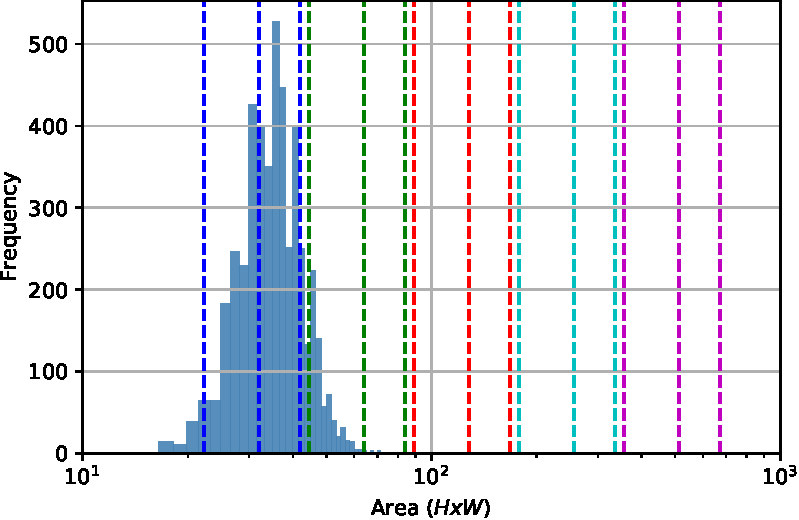
\includegraphics[width=0.45\textwidth]{figures/ch3/fig2_1.pdf}
    \label{fig2_1}
  }
  \subfigure[Validation dataset.]{
    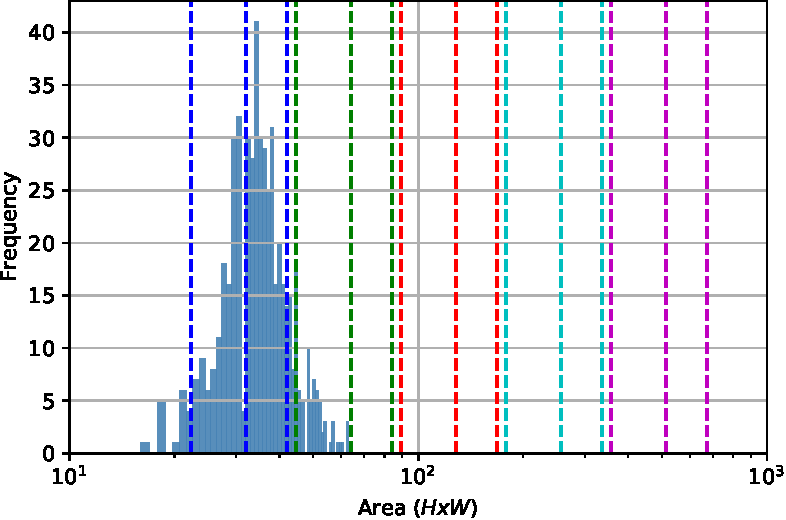
\includegraphics[width=0.45\textwidth]{figures/ch3/fig2_2.pdf}
    \label{fig2_2}
  }
  \caption{The annotation boxes' area distribution, along with the scaled optimised anchor boxes. It can be seen that the anchors of the last 3 layers are almost redundant.}
  \label{fig2}
\end{figure}

\subsection{Hyper-parameter Selection}
The IoU threshold to consider a detection as a true positive was set equal to $IoU_{th} = 0.2$ (as in \cite{bargoti2017deep} to perform valid comparisons). The confidence score for the proposed detections was set as $p(c_i) > 0.05$ and the $\text{NMS}_{th}$ was set equal to 0.3, as it found out to be the best after experimentation. To save computation time the maximum proposed detections allowed was set to be 100. 

Finally, concerning the loss function, tweaking $\alpha$ and $\gamma$ did not yield any difference in performance, so the default parameters $\alpha=0.25$ and $\gamma=2$ remained unchanged. A notable remark is that the loss function was found to be very unstable during training. The reason was that the normalisation parameters take values equal to the total number of the instances in the image. This behaviour is a result of the increased variance exhibited by the Fruit/Img., as can be seen in \tref{tab1}. To tackle this issue, the normalisation factor was modified, taking values from an exponential moving average of the total instances in the samples.
 
\section{Proposed Architectures}
RetinaNet network exploits the inherent multi-scale, pyramidal hierarchy of the backbone network making predictions in multiple scales. Deeper layers capture higher levels of abstraction, making coarser feature maps semantically stronger comparing to finer feature maps. Rougher feature maps are also useful for predicting bigger objects due to their receptive field. \fref{fig1} shows that detection from higher pyramidal levels might be redundant. 

The proposed architectures explore:
\begin{itemize}
 \item the depth impact of the backbone through the VGG11, VGG13, VGG16 and VGG19 architectures
 \item and the topology of the side network of RetinaNet, responsible for the detection part.
\end{itemize}

Inference time, network's number of parameters and the need in computational and memory resources can be further reduced through an optimised network, that achieves maximum performance at the same time.

\textbf{Architectures}
\begin{itemize}
 \item{\textbf{Original}:}\label{arch_1} 
The first architecture, original RetinaNet, uses 5 pyramidal levels (P3,P4,P5,P6,P7) for prediction. P3, P4 and P5, are obtained via lateral connections right after the corresponding VGG blocks (reduced in a fixed depth of $\times256$) and are semantically enhanced as shown in the right-left pathway in \fref{fig3}. P6 and P7 are obtained from single $3\times3$ strided convolutions after the last VGG convolutional block. Finally, a common predictor and box regressor makes predictions from each layer.

\begin{figure}[!htb]
  \centering
  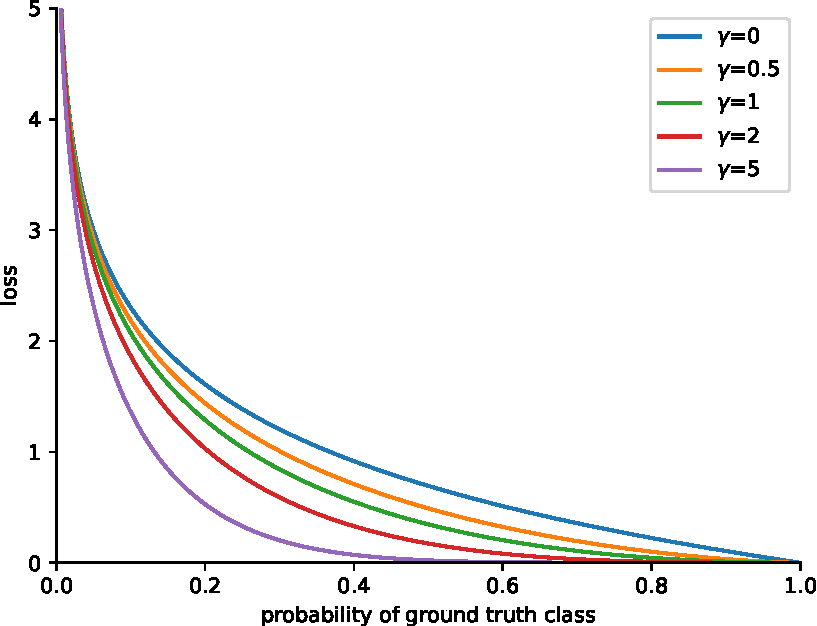
\includegraphics[width=0.5\textwidth]{figures/ch3/fig3.pdf}
  \caption{The original RetinaNet pipeline. No. of parameters: 8.7M (without VGG).}
  \label{fig3}
\end{figure} 

 \item{\textbf{$\text{P}_3\text{P}_4\text{P}_5$}:}\label{arch_2}
The second architecture follows the original RetinaNet structure, without utilising P6 and P7 at all. P3, P4, P5 still follows the upsampling-merging technique. The difference with the original architecture is that it is incapable of detecting objects ranging  between $200^2$ - $700^2$ pixels.

\begin{figure}[!htb]
  \centering
  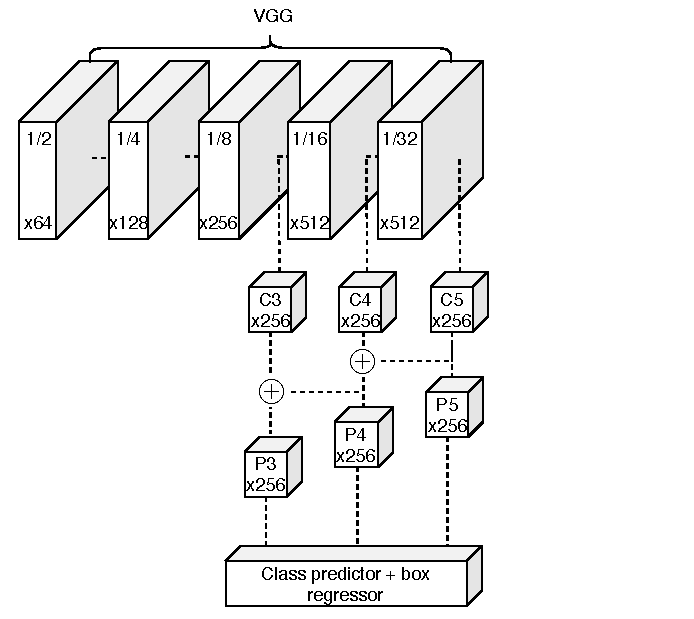
\includegraphics[width=0.5\textwidth]{figures/ch3/fig4.pdf}
  \caption{RetinaNet - $\text{P}_3\text{P}_4\text{P}_5$: A slightly different version of RetinaNet without using P6 and P7 . No. of parameters: 6.9M (without VGG).}
  \label{fig4}
\end{figure} 

 \item{\textbf{$\text{P}_\text{i}\text{Multi}$}:}\label{arch_3}
The next architecture is similar to the previous. However, instead of sharing common classification and regression heads, each $P_i$ has separate classifiers and regressors with unshared parameters. This architecture is much more computationally and memory expensive, however, the reasoning behind this deployment is to investigate if by attaching multiple classification and regression heads, there is any gain in performance.

\begin{figure}[!htb]
  \centering
  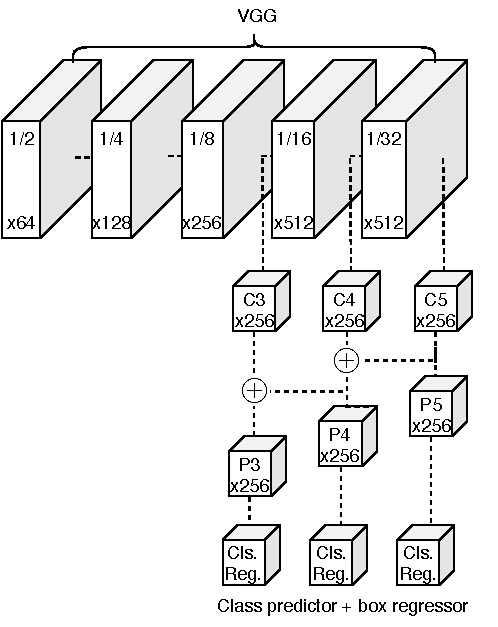
\includegraphics[width=0.5\textwidth]{figures/ch3/fig5.pdf}
  \caption{RetinaNet - $\text{P}_\text{i}\text{Multi}$: A modified Architecture - 2 with separate classification. and regression submodel. No. of parameters: 16.6M (without VGG).}
  \label{fig5}
\end{figure} 

 \item{\textbf{$\text{C}_\text{i}\text{Reduced}$}:} 
Finally, the last configuration is the lightest among all. It utilises only the reduced in depth feature maps obtained right after block 3, block4 and block 5 from VGG by attaching common classifier and box regressor heads. It is inspired by the SSD (\cite{liu2016ssd}), but is considerably lighter, as it skips the extra layers after block 5 of the VGG network.

\begin{figure}[!htb]
  \centering
  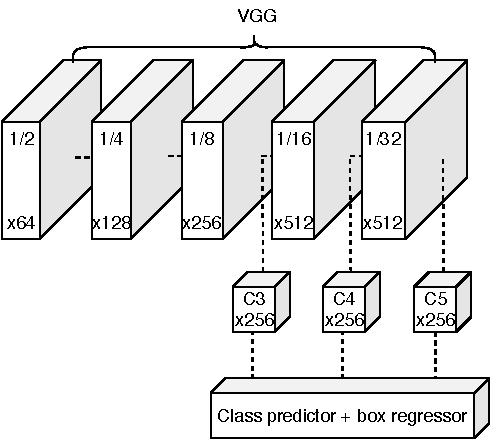
\includegraphics[width=0.5\textwidth]{figures/ch3/fig6.pdf}
  \caption{RetinaNet - $\text{C}_\text{i}\text{Reduced}$: The lightest architecture, inspired by the SSD, but more much shallower. No. of parameters: 5.1M (without VGG).}
  \label{fig6}
\end{figure} 

\end{itemize}

